\chapter{Gas naturale (\textit{NG})}
Il gas naturale � una materia prima alternativa a petrolio, soprattutto nella produzione di idrogeno e di gas di sintesi (una miscela di $H_2$ e $CO$) mediante steam reforming. \'E costituito prevalentemente da metano ($CH_4$), ma pu� contenere anche frazioni significative di paraffine ($C_2$ e $C_3$). In base al quantitativo di condensabili ($C_2$ e $C_3$) presenti si distingue in \textit{dry gas} e \textit{wet gas}, inoltre se la presenza di $CO_2$ e $H_2S$ � significativa il gas si dice \textit{acido}.

Il gas naturale si pu� trovare in giacimenti associato al petrolio, nel qual caso i costi di estrazione sono minimi, mentre per i pozzi di \textit{NG} non associati i costi sono maggiori, poich� non vi sono materie di maggior pregio da estrarre con esso.

\section{Purificazione}
La purificazione del metano da $H_2S$ pu� essere svolta usando un assorbimento chimico o fisico. L'assorbimento \textit{chimico} viene scelto quando le quantit� di acido solfidrico da rimuovere sono basse, mentre per grandi quantitativi di acido da asportare si utilizza l'assorbimento \textit{fisico}.

L'assorbimento chimico viene condotto in colonne di assorbimento, alla cui base viene inviato il gas da trattare, mentre dalla testa si inviano soluzione alcaline di etanolammine o carbonato di potassio ($K_2CO_3$). \'E un trattamento altamente selettivo, ma se il quantitativo di acido solfidrico � troppo elevato si ha saturazione del solvente con conseguente perdita di attivit�.

L'assorbimento fisico viene preferito quando si hanno elevate quantit� di gas da trattare con elevate concentrazioni di $H_2S$. L'operazione viene condotta in una colonna di assorbimento e il solvente � costituito da \textit{N-metil-pirrolidone} glicoli e metanolo. L'utilizzo di questi solventi da una minore selettivit�, ma al contempo non ha problemi di saturazione del solvente. La fase successiva del processo � la rigenerazione del solvente in un colonna di stripping.

Sono possibili anche purificazioni tramite assorbimento ossidativo a zolfo (adatto a piccole correnti da trattare) o assorbimento su letti solidi (costituiti da ossidi di ferro, zinco o carboni attivi), che per� devono essere rigenerati.

In tutti questi casi il gas naturale viene trattato in pressione in modo da favorire il fenomeno di assorbimento, con scelta del meccanismo in base alla portata e alla concentrazione dei gas, come visibile in \figurename~\ref{fig:NG:Adsorbimento}

\begin{figure}[htbp]
	\centering
		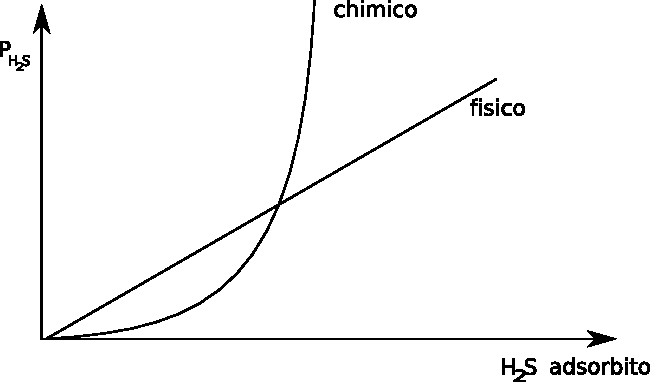
\includegraphics[width=0.60\textwidth]{image/NGAdsorbimento.pdf}
	\caption{Confronto tra assorbimento \textit{chimico} e \textit{fisico} a diverse concentrazioni di $H_2S$}
	\label{fig:NG:Adsorbimento}
\end{figure}

\section{Trasporto}
Il trasporto del gas naturale dal punto di estrazione ai punti di consumo pu� essere effettuata tramite gasdotti o, una volta liquefatto, con navi metaniere. Attualmente il 75\% del \textit{NG} viene trasportato per mezzo di gasdotti, in cui il gas si trova a una pressione di circa 80MPa, mentre il restante viene trasportato via mare.

La scelta del tipo di trasporto da effettuare dipende, tanto dalle infrastrutture presenti nel luogo di estrazione (presenza o meno di gasdotti), quanto dalla distanza da percorrere, infatti per liquefare il gas naturale � necessario portarlo (e conservarlo) a una temperatura di circa -160�C, con un costo energetico di circa 6MJ/kg. Il metodo di scelta del tipo di trasporto pu� ben essere rappresentata in \figurename~\ref{fig:NG:Trasporto}. Come � evidente le spese per il trasporto su \textit{pipeline off-shore} (fuori costa, in mare) crescie pi� rapidamente che non il trasporto \textit{on-shore}.

\begin{figure}[htbp]
	\centering
		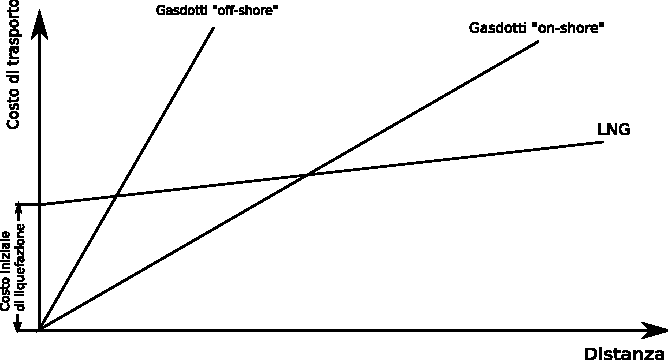
\includegraphics[width=0.60\textwidth]{image/NGTrasporto.pdf}
	\caption{Costo per le diverse tipologie di trasporto in funzione della distanza}
	\label{fig:NG:Trasporto}
\end{figure}

Il quantitativo di \textit{NG} trsporto su navi metaniere � di circa $125000m^3$, in cui il metano � stoccato a -160�C in forma liquida ($d = 424kg/m^3$) con una concentrazione circa 600 volte maggiore che il gas allo stato gassoso; la portata nei gasdotti � di $2-4 \cdot 10^6 Nm^3/h$.

Un'alternativa al trasporto del gas naturale in altri siti � l'utilizzo in loco per la produzione di metanolo che costitusce un prodotto di maggior pregio ed � pi� facilmente trasportabile.